\newchapter{Musket Ball: DM Implications}{Musket Ball Cluster: Dark Matter Implications}{Musket Ball Cluster: Dark Matter Implications}
\label{chapter:4}

\noindent Portions of this chapter were originally published in the article titled \emph{Discovery of a Dissociative Galaxy Cluster Merger with Large Physical Separation} which was published in the March 2012 issue of the Astrophysical Journal Letters (Volume 747, pp. L42). \\

\section{Introduction}

As introduced in \S\ref{section:DMconstraintWithMergers} there are four methods of constraining $\sigma_{\rm SIDM}$ with observations of dissociative mergers.
In this chapter we apply two of those methods to observations of the Musket Ball Cluster.
First we will consider the gas-DM offset, and second we will consider the galaxy-DM offset.
As discussed in \S\ref{section:DMconstraintWithMergers} these two methods are believed to be the most robust.
In both cases we will depend on the WL measurements to ascertain the location of the DM.
The galaxy location will be determined from optical spectroscopic and photometric observations of the galaxies.
The gas location will be determined from X-ray observations of the cluster.
Of the three location measurements... (the galaxy is the most difficult???)

We note that the exercise of comparing the galaxy-WL offset will be incomplete in this analysis, since simulations of mergers with varying $\sigma_{\rm SIDM}$ are necessary to turn any observed offset (or lack of offset) into a quantitative constraint on$\sigma_{\rm SIDM}$ (see \S\ref{section:DMgalaxyOffsetIntro}). 
However we chose to present the observation portion of this analysis for two reasons.
First, it is a necessary first step towards applying this constraint.
Secondly, if a significant offset is observed then one could still conclude that $\sigma_{\rm SIDM}$>0, which would be a significant finding since this would imply that DM is self-interacting via a new force.

For both the gas-DM offset and galaxy-DM offset methods the primary measurements necessary are the location of the galaxies (\S\ref{section:GalaxyLocation}), gas (\S\ref{section:GasLocation}), and DM (\S\ref{section:WLLocation}).
Much of this chapter will focus on how there measurements are made with the later sections (\S\ref{section:GasWLOffset} and \S\ref{section:GalaxyWLOffset}) discussing the offset measurement and their implications for $\sigma_{\rm SIDM}$.

\subsection{Location Estimation}\label{section:LocationEstimation}
For the original work of \citet{Dawson:2012dl} (see Chapter 2) I estimated the weak lensing subcluster positions and errors on their positions by using the location of the peak signal in a region and estimated the variance on the peak by measuring the peak location of each bootstrap iteration within the selected region.  
For this chapter, rather than using the location of the peak and variance of the peak, I have adopted an iterative centroid estimation scheme, similar to \citet{Randall:2008hs} (and often used in N-body simulations). 
I begin by calculating the centroid of a large aperture that encompasses one subcluster, but excludes the other.
I then decrease the aperture, recenter on the previously calculated centroid, and estimate the centroid of the new aperture.
This process is repeated until the aperture is decreased to a radius of $\sim200$\,kpc.
To estimate the uncertainty on the location I perform this process on each iteration of a random bootstrap sample map, resulting in a array of centroid values.
 The uncertainty on the location is then inferred from the variance of this array of centroid values.


%-------------------------------------------------------
%-------------------------------------------------------
%-------------------------------------------------------
\section{Galaxy Location}\label{section:GalaxyLocation}

Galaxies are expected to populate dark matter subhalos (Yao et al REF) and from dark matter simulations these subhalos are found to be the building blocks of clusters.
Thus galaxies are believed to be tracers of the underlying dark matter distribution.
Evidence for this is found across all cosmological mass scales from dwarf speroidals (REF), to galaxies (REF ami), groups (REF Matt), clusters (REF), and large scale structures (REF filament work).
So the location of galaxies is expected to coincide with the location of the DM in $\Lambda$CDM, to within some amount of intrinsic scatter.
It is precisely this phenomenon that we wish to challenge with observations of merging galaxy clusters, since for some non-zero $\sigma_{\rm SIDM}$ the location of the galaxy population is not expected to coincide precisely with the underlying DM distribution.
As far as the location of the galaxy population (i.e. center) is concerned there are three main challenges.
First, there are many ambiguous definitions the galaxy population location and these definitions often result in different estimates, sometimes even outside the uncertainty of each measurement \citep{George:2012uo}.
Second, due to inherent observational limitations in determining galaxy positions and velocities it can be difficult to determine which galaxies are members of a given DM halo (and expected tracers of that DM halo).
Third, even if galaxies are a fair sample of the underlying DM halo there are often only a few hundred to trace a given halo.
Thus a certain amount of intrinsic scatter between the location of the galaxy population and the underlying DM distribution is to be expected simply due to Poisson noise.
This is in addition to the intrinsic scatter that is due to galaxies being dynamic tracers of an ever evolving DM halo. 

\subsection{Definition of Galaxy Location}

There are many different definitions of the location of the galaxy population.  
One that is commonly used is simply defining the location to be at the position of the brightest cluster galaxy \citep[e.g.][]{Gladders:2000ca, Koester:2007en, Hao:2010kz}.
This method is often straightforward and for relaxed systems seems to agree well with other cluster location measures such as the X-ray location \citep{Sheldon:2001kk, Koester:2007en, Sanderson:2009hi,George:2012uo}.
In relaxed cool-core clusters the location of the BCG is found to agree with the location of the gas to within $\leq$15\,kpc, however in non-cool core and potentially disturbed clusters the locations can be offset by $\sim100$\,kpc \citep{Sanderson:2009hi}.
It is unclear in the case of the \citet{Sanderson:2009hi} non-cool core clusters which if either location is a better tracer of the DM location.
The disadvantage of the BCG location method is that not all clusters have a dominant BCG ($\sim$1--2 magnitudes brighter than the next brightest cluster galaxy).
This is the case with the Musket Ball Cluster.
In such cases the BCG is found to provide an unreliable location \citep[see e.g.][]{George:2012uo}

An obvious alternative to choosing a single galaxy to represent the central location of the population is to use the whole or a subsample of the galaxy population to estimate a central location.
This is often done by estimating the weighted galaxy centroid \citep[e.g.][]{Berlind:2006dy, Carlberg:2001fp, Jee:2011we, George:2012uo},

\begin{equation}
\vec{x}_{\rm centroid} = \frac{\sum_{i=1}^N w_i\vec{x}_i}{\sum_{i=1}^N w_i},
\end{equation}\label{equation:WeightedCentroid} 
where $\vec{x}_{\rm centroid}$ is the calculated centroid coordinates (right ascension and declination in the case of observations) for a population of $N$ galaxies with $\vec{x}_i$ the coordinate of galaxy $i$ and $w_i$ is the weight assigned to that galaxy.
In the case of a simple galaxy number density centroid $w_i$=1.
It is common to weight galaxies by their luminosity or stellar mass.
\citet{George:2012uo} find that for groups of galaxies centroid based location estimates typically have larger uncertainties ($\sim50$\,kpc) and appear to be offset more from the underlying DM distribution than BCG (or in their case brightest group galaxy, BGG) location estimates.
However, it is important to note that this work was performed on groups of galaxies (typically $\sim$1 order of magnitude less massive and with $\sim$1 order of magnitude fewer galaxies than galaxy clusters).
Since the the centroid measurement error will scale proportional to the number of member galaxies like $N^{-1/2}$, this will result in a noisier estimate in the case of galaxy groups.
In support of this reasoning, \citet{Jee:2011we} found that clusters in their sample with high lensing signal (i.e. more massive) that the galaxy centroids ``agree well with the mass peaks''.
However in the same sample they find that clusters where the lensing signal is weak they observe offsets >20'' between the mass and galaxies.
The \citet{George:2012uo} and \citet{Jee:2011we} results suggest that the systematic offset of the galaxy centroid estimate can be a strong function of the mass of the group or cluster.
Because the Musket Ball Cluster does not have a dominant BCG in either subcluster we will adopt the centroid location estimate method.
Finally smoothing based methods are an alternative population based location estimate, and while not used in this dissertation they are worth future consideration.
Typically in these methods the projected distribution of galaxy members are smoothed by a signal matched smoothing kernel and then the peak of this smoothed distribution is used as the location \citep[see e.g.][]{Merritt:1994fc, Gonzalez:2002kl, Randall:2008hs}.


\subsection{Cluster Membership}\label{section:ClusterMembership}

Another major challenge in determining the galaxy population location is separating the sample of galaxies that are gravitationally bound to a DM halo from foreground and background galaxy samples.
This contamination of the cluster sample by fore/background galaxies and the dilution of the cluster sample by improperly assigning cluster members to the fore/background galaxy sample will both act to decrease the signal-to-noise of the galaxy centroid measurements.
In the case of isolated clusters these effects should not induce a directional bias in the centroid measurement, however in the case of merging clusters it is possible to induce such a bias.
In a dissociative merger the two subclusters are often in close proximity to one another, both in projected space (often within each others' virial radii) and redshift space (often within each others' velocity dispersion).
Thus the galaxy centroid estimate of one subcluster will be biased away from the true galaxy centroid of that subcluster towards the other subcluster.
This may cancel to some degree with a similar directional bias in the WL estimate of the DM location (see \S\ref{section:WLLocation}) although studies of these relative biases have not been performed.  

The challenge in determining cluster galaxy membership lies with the inherently limited observational information that one can obtain of galaxies.
While it is relatively easy to constrain the projected position of galaxies to sub-arcsecond precision, it is much more difficult to constrain the position of galaxies along the line-of-sight.
The best than can be done in this regard are spectroscopic redshifts of the galaxies, which can often constrain the line-of-sight velocities to a few km\,s$^{-1}$ \citep[in the case of a 1200 line mm$^{-1}$ grating with resulting resolution of $\sim 1\,\AA$; see e.g.][]{Dawson:2012ub}.
However, spectroscopic surveys are observationally intensive often requiring a large amount of time (a few nights) on large telescopes ($\gtrsim$5\,m)\footnote{Take for example the completeness of the spectroscopic survey carried out on the Musket Ball Cluster (see Figure \ref{figure:PhotozSpeczMagDist}) over 1.5 nights using the DEIMOS multi-object spectrograph on the Keck 10\,m telescope.}.
Thus, many astronomers have developed and used membership identification methods that only require photometric galaxy surveys since these are capable of surveying many more galaxies is a much shorter amount of time even on smaller telescopes \citep[e.g. the DLS,][]{Wittman:2002cp}. 

Even in the idealized case of having spectroscopic redshift information for all galaxies two major problems remain when estimating galaxy cluster membership in dissociative mergers.
The first challenge is the ``finger of god effect''.
The typical velocity dispersion of cluster galaxies is $\sim$1000\,km\,s$^{-1}$, and since a velocity difference ($\Delta v$) is related to a redshift difference ($\Delta z$) by,
\begin{displaymath}
\Delta z = \frac{\Delta v (1+\bar{z})}{c},
\end{displaymath}
the member galaxies of a cluster will often have $\Delta z\sim$0.015 (for a cluster at $z$=0.5).
This corresponds to a Hubble flow separation of $\sim$30\,Mpc, which is roughly an order of magnitude larger than the cluster size.
Thus it is nearly impossible to distinguish between cluster galaxies and projected fore/background galaxies within $\sim\pm$30\,Mpc of the cluster redshift.
Fortunately clusters are $\sim$20-70 times more dense than other cosmic structures \citep[e.g. filaments, walls and voids;][]{AragonCalvo:2010cq}, thus this should not be a dominant source of noise.
Potentially more problematic is the second challenge to determining cluster membership which is specific to dissociative mergers.
This challenge is that the typical relative merger velocity of the two subclusters in a dissociative merger is of order the velocity dispersion of each subcluster.
Thus it is difficult to disengangle the members of each subcluster.
While similar to the ``finger of god effect'' this effect is potentially more serious since the central densities of each subcluster are of the same order of magnitude; for mergers just after first pass through this will be more of an issue than further progressed mergers with larger projected separations between the two subclusters.
As previously mentioned this effect can potentially lead to a directional bias in the galaxy centroid estimate.
 
In the less ideal scenario where limited spectroscopic information is available we must attempt to determine cluster membership with only photometric data.
In cases where multi-band ($\gtrsim 4$) observations have been carried out photometric redshift estimates can be made for most of the galaxies detected with moderate signal-to-noise ($\sim$20).
However, photometric redshift uncertainties ($\sigma_{\rm z-phot}\sim$0.07(1+$z_{\rm phot}$)) are typically many orders of magnitude larger than spectroscopic redshift uncertainties and a couple orders of magnitude larger than the typical redshift velocity dispersion of a cluster.
Thus, even if a galaxy has the exact same $z_{\rm phot}$ as the cluster there is still considerable uncertainty in whether that galaxy is a member of the cluster.
In extreme cases of extreme photometric coverage (30-bands from ultraviolet to infrared) it is possible to identify 92\% of cluster member (down to the limiting magnitude) with 84\% purity \citep{George:2011kv}.
It is often the case that there is not enough photometric coverage of a system to obtain reliable photometric redshifts and astronomers have used prior information about the properties of galaxies (e.g. luminosity, color, and stellar mass)  in cluster environments to improve membership identification \citep[see][for a review]{George:2012uo}. 

\subsection{Galaxy Location Poisson Noise}

The third challenge is estimating the galaxy population location is that there are often only a few hundred galaxies that trace a given DM halo's potential.
Thus a certain amount of intrinsic scatter between the location of the galaxy population and the underlying DM distribution is to be expected simply due to Poisson noise.
This source of galaxy location noise is often at direct odds with the noise from galaxy cluster membership.
As one attempts to increase the number of cluster members (i.e. completeness) used in the centroid calculation to reduce they Poisson noise, they often must sacrifice purity (fraction of true cluster members to the assumed number of cluster members) which increases the noise due to cluster membership error.
For example, the systematic error due to contamination can be decreased by placing strict membership requirements, e.g. only using galaxies that have spectroscopic redshifts within some small factor (e.g. 3) of the cluster velocity dispersion.
However this will reduce the number of galaxies that are used to estimate the centroid and the Poisson noise will increase.
At the outset there is not a clear what the optimal choice of membership selection criteria should be to minimize the joint membership noise and Poisson noise, however it is conceivable that this could be empirically determined for a given dataset.

\subsection{Estimating the Musket Ball Cluster's Galaxy Location}

\subsubsection{Musket Ball Cluster Galaxy Location Data}

Most of the available data to constrain the galaxy locations of the Musket Ball Cluster is presented in detail in Chapters \ref{chapter:2} and \ref{chapter:3}, however we review some of the important information now.
Because the Musket Ball Cluster is within the DLS \citep{Wittman:2002cp} it has 4-broad-band photometry ($BVRz$) to limiting magnitudes of $\sim26$ (see e.g. Figure \ref{figure:PhotozSpeczMagDist}).
Additionally we also observed the cluster in three medium-width optical bands ($g,h,$ and $i$ from the BATC filter set), bracketing the redshifted $4000$\,\AA\, feature.
This coverage has enabled photometric redshifts to be estimated for most of the galaxies in the cluster field with $R\lesssim26$, however photometric errors increase for fainter galaxies and this in turn increases the photometric redshift uncertainty.  
For the DLS it is found that $\sigma_{\rm z-phot}\approx$0.07(1+$z_{\rm phot}$ for galaxies with $R\leq24$; photo-z's become unreliable fainter than $R\sim$24 \citep{Schmidt:2013ig}.
Thus in all our analyses of the Musket Ball Cluster's galaxy locations we only use galaxies with$R\leq24$.

\begin{figure}
	\centering
	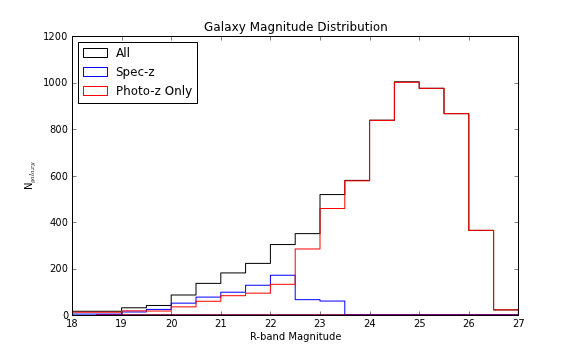
\includegraphics[width=5in]{Chapter4/AnalysisFiles/magdist.png}
	\caption[Musket Ball Cluster spectroscopic and photometric magnitude distribution.]{
	The Musket Ball Cluster spectroscopic (blue) and photometric (red) galaxy magnitude distribution in the $\sim$15'$\times$15' spectroscopic survey area.
	While the DLS photometric survey is complete to $R\sim26$ photometric redshifts are only reliable to $R\sim24$.
		}
	\label{figure:PhotozSpeczMagDist}
\end{figure}

In addition to the deep photometric data we have carried out an extensive spectroscopic survey of the Musket Ball Cluster (see \S\ref{section:MusketBallSpectroscopy} and \S\ref{sec_MBCzcat}).
We have obtained a sample of 738 spectroscopically confirmed galaxy redshifts within an $\sim 18\arcmin \times 18\arcmin$ area centered on the Musket Ball Cluster ($139.05\deg$, $+29.85\deg$).
This survey covers a significant fraction of the galaxies in the area brighter than $R=23$, see Figure \ref{figure:PhotozSpeczMagDist}.
This spectroscopic sample has also provided important information of the accuracy of the photometric redshifts, see Figure \ref{figure:photzVSspecz}, in particular their accuracy of determining cluster galaxy membership.

\begin{figure}
\centering
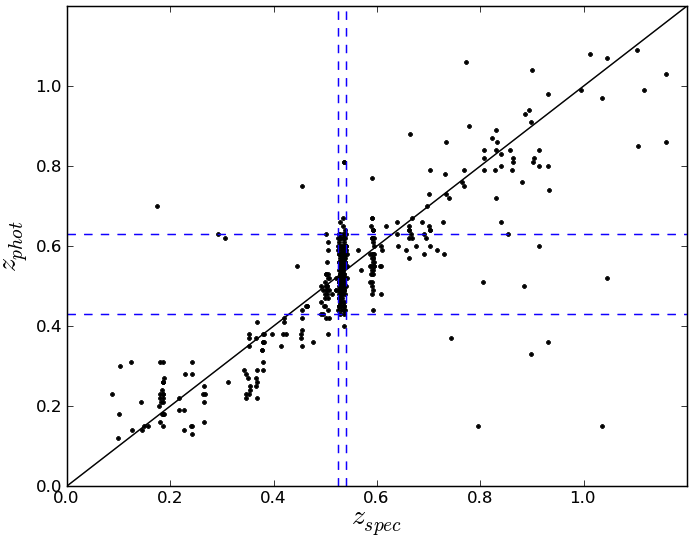
\includegraphics[width=5in]{Chapter4/photVSspec.png}
\caption[Spectroscopic verses photometric redshift for the Musket Ball Cluster.]{
Spectroscopic redshifts verses photometric redshift estimates for the galaxies observed in the Musket Ball Cluster $R<$23.5 magnitude limited survey (discussed in Chapter \ref{chapter:2} and \S\ref{sec_MBCzcat}).
The horizontal dashed blue lines highlight the 0.43$\leq z_{\rm phot} \leq$0.63 range.
63\% of the surveyed galaxies within this range are cluster members.
The verticle dashed blue lines highlight the 0.525$\leq z_{\rm spec} \leq$0.54 or three times the cluster velocity dispersion.
}
\label{figure:photzVSspecz}
\end{figure}


\subsubsection{Fully Probabilistic Membership Determination}

The first of two membership determination methods applied to the Musket Ball Cluster is rooted in the desire to treat both spectroscopic and photometric redshift samples in a consistent manner. 
This method slightly favors minimizing the Poisson noise while still trying to address the systematic contamination error. 
The basic approach is to assign weight to each galaxy roughly based on its probability of being a cluster member.
This weight is defined as the inner product of the redshift probability density function (PDF) of a galaxy $p(z)_i$ and the redshift velocity dispersion of the cluster (assumed to be Gaussian),
\begin{equation}
w_i = \int_{0}^{\infty} p(z)_i \frac{1}{\sigma_{\rm vdisp}\sqrt{2\pi}}e^{\frac{-(z-z_{\rm cluster})^2}{2\sigma_{\rm vdisp}^2}}\mathrm{d}z,
\label{equation:genericz_weight}
\end{equation}
where $\sigma_{\rm vdisp}$ is the redshift velocity dispersion of a cluster a redshift $z_{\rm cluster}$.
Since the redshift uncertainty of a spectroscopically observed galaxy with $z_{\rm spec_{i}}$ is $\ll \sigma_{\rm vdisp}$ and its redshift PDF can be treated as a delta function and Equation \ref{equation:genericz_weight} reduces to
\begin{equation}
w_i = \frac{1}{\sigma_{\rm vdisp}\sqrt{2\pi}}e^{\frac{-(z_{\rm spec_{i}}-z_{\rm cluster})^2}{2\sigma_{\rm vdisp}^2}}.
\end{equation}\label{equation:specz_weight}
Under the assumption of Gaussian photometric redshift errors ($\sigma_{\rm z-phot_{i}} \approx \bar{\sigma}(1+z_{\rm phot_{i}})$; $\bar{\sigma}$=0.07 for the Musket Ball Cluster) Equation \ref{equation:genericz_weight} takes the form
\begin{equation}
w_i = \int_{0}^{\infty} \frac{1}{\sigma_{\rm z-phot_{i}}\sqrt{2\pi}}e^{\frac{-(z-z_{\rm phot_{i}})^2}{2\sigma_{\rm z-phot_{i}}^2}} \frac{1}{\sigma_{\rm vdisp}\sqrt{2\pi}}e^{\frac{-(z-z_{\rm cluster})^2}{2\sigma_{\rm vdisp}^2}}\mathrm{d}z.
\label{equation:photoz_weight}
\end{equation}

When estimating the galaxy centroid these weights are simply used in conjunction with Equation \ref{equation:WeightedCentroid}.
The bootstrap realizations used in the centroid uncertainty estimate are handled in a slightly different but equivalent manner.
Using these weights we form a cumulative normalized weight distribution for all the galaxies with $R<24$ and within a 9' by 9' region surrounding the Musket Ball Cluster (see Figure \ref{figure:NormWeightDist}).
During the bootstrap sampling process a random number between 0 and 1 is drawn from a uniform distribution, where this random number intersects the weight distribution determines the randomly selected galaxy.
Beyond this weighted draw with replacement the bootstrap uncertainty analysis is standard in all regards.

\begin{figure}
\centering
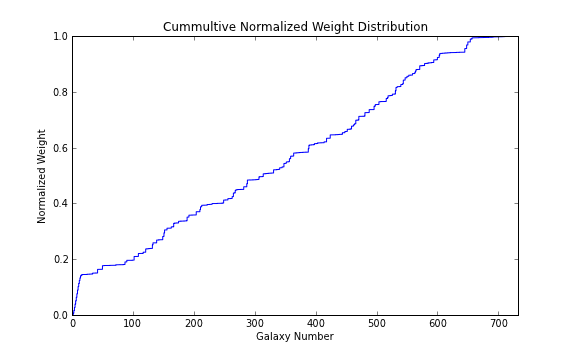
\includegraphics[width=4in]{Chapter4/AnalysisFiles/cumnormwghtdist.png}
\caption[Probabilistic scheme; cumulative normalized weight distribution for galaxies being in the Musket Ball Cluster.]{
The resulting cumulative weight distribution for all the galaxies with $R<24$ and within a 9' by 9' region surrounding the Musket Ball Cluster.
This distribution is used to perform a weighted random draw of cluster galaxies (e.g. the green distribution of Figure \ref{figure:ProbWeightDist}) for the galaxy centroid bootstrap analysis.
This distribution is determined by Equations \ref{equation:specz_weight} and \ref{equation:photoz_weight}.
During the bootstrap sampling process a random number between 0 and 1 is drawn from a uniform distribution, where this random number intersects the weight distribution determines the randomly selected galaxy.
Note that the catalog is sorted such that the spectroscopic members are first, thus the noticeably steeper slope for the early galaxy numbers.
}
\label{figure:NormWeightDist}
\end{figure}

Comparing the galaxy redshift distribution of a random bootstrap realization with the redshift distribution of the parent population (Figure \ref{figure:ProbWeightDist}) it is apparent that the fully probabilistic membership determination scheme still includes a large number of galaxies with photometric redshift estimates well outside the cluster redshift velocity dispersion ($z_{\rm cluster}\pm\sigma_{\rm vdisp} \approx 0.53\pm0.004$).
The reason for this is simply that the photometric redshift uncertainties are so large compared to all other pertinent redshift scales.
Thus, galaxies that have the exact same photometric redshift as the cluster are not weighted dramatically more than galaxies with photometric redshift estimates well in front of or behind the cluster.
Take for example two photometric redshift galaxies, one at the cluster redshift ($z=0.53$) and one well behind the cluster at $z_{\rm phot}=0.79$.
According to Equation \ref{equation:photoz_weight} the galaxy with $z_{\rm phot}=0.53$ will have a weight of 3.7 while the galaxy with $z_{\rm phot}=0.79$ will have a weight of 0.37.
Since even in this small projected region around the Musket Ball Cluster the number of fore/background galaxies outnumbers the cluster member, this probabilistic weighting scheme will always result in a significant amount of contamination.
This is likely why \citet{George:2011kv} base their probability of cluster membership both on the expected distribution of the cluster members as well as the field.
Such a method is worth considering for future work but is currently beyond the scope of this dissertation.
Instead we will use an empirical based method to determine our weighting scheme of cluster membership. 


\begin{figure}
\centering
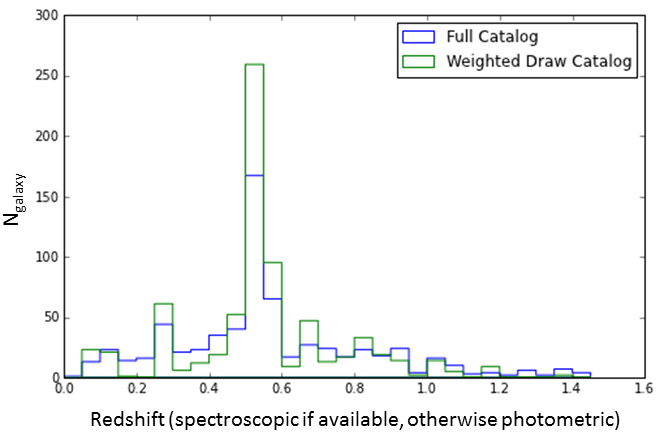
\includegraphics[width=4in]{Chapter4/AnalysisFiles/zdist_randomweightdraw_reformat.png}
\caption[Comparison of parent galaxy redshift distribution with weighted random draw distribution.]{
The redshift (spectroscopic if available, otherwise photometric) distribution of all the galaxies in a 9'$\times$9' area surrounding the Musket Ball Cluster with $R<$24 (blue); and a single bootstrap sample (green) drawn from the fully probabilistic weighted distribution (Figure \ref{figure:NormWeightDist}).
While the probabilistic scheme does work to increase the number of galaxies selected at the cluster redshift ($z=0.53$) it still selects a disproportionate number of galaxies with photometric redshifts outside of the cluster redshift; see that in Figure \ref{figure:photzVSspecz} only 1 galaxy of our spectroscopic survey sample with $z_{\rm phot}$>0.7 is actually at the cluster redshift and only 1 galaxy with $z_{\rm phot}<$0.43 is at the cluster redshift.
}
\label{figure:ProbWeightDist}
\end{figure}


\subsubsection{Empirically Based Membership Determination}\label{section:EmpiricalWeightScheme}

The second method of membership determination is considerably less elegant but more empirically based and aims higher cluster membership purity.
If a galaxy has a spectroscopic redshift within the 3$\sigma_{\rm vdisp}$ range of the cluster redshift (0.525$<z_{\rm spec}<$0.54 for the Musket Ball Cluster) it is given a weight of 1\footnote{
Note that this ignores the ``finger of god effect'', although since it is reasonable to assume that the number of cluster galaxies should dominate the number of fore/background galaxies within $\pm$30\,Mpc of the cluster redshift this effect should not dominate the centroid uncertainty.}
If galaxies only have a photometric redshift and that happens to be within the range 0.43$\leq z_{\rm phot} \leq$0.63 (approximatly the Musket Ball Cluster redshift $\pm sigma_{\rm z-phot}$) they are given a weight of 0.63.
All remaining galaxies are given a weight of 0.
The cumulative normalized weight distribution function for this weighting scheme is shown in Figure \ref{figure:NormPenaltyWeightDist}.

The motivation behind the photometric redshift weight of 0.63 comes from our magnitude limited redshift survey\footnote{The survey was magnitude limited in regards to the fact that we targeted any galaxy with $R$<23.5, if galaxies had a 0.43$\leq z_{\rm phot} \leq$0.63 there likelihood of being target was twice that of other galaxies. This should not bias the conclusions of this section since we are limiting ourselves to considering just the range 0.43$\leq z_{\rm phot} \leq$0.63. Figure \ref{figure:PhotozSpeczMagDist}.}
of the Musket Ball Cluster.
We obtained 355 high quality spectra of galaxies with 0.43$\leq z_{\rm phot} \leq$0.63 and 210 of these spectroscopic redshifts were between 0.525$<z_{\rm spec}<$0.54, see for example Figure \ref{figure:photzVSspecz}.
This translates to a purity of 63\%.
Note that this photometric redshift range should result in a cluster membership completeness of 95\%.

\begin{figure}
\centering
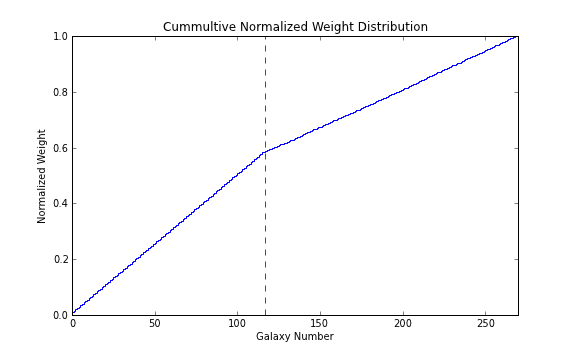
\includegraphics[width=4in]{Chapter4/AnalysisFiles/cumnormwghtdist_zclip_photozpenalty.png}
\caption[Photometric redshift penalization scheme; cumulative normalized weight distribution for galaxies being in the Musket Ball Cluster.]{
The photometric redshift penalization scheme cumulative normalized weight distribution (blue step curve) for galaxies being in the Musket Ball Cluster. 
Galaxies that are spectroscopically confirmed cluster members (0.525$\leq z_{\rm spec} \leq$0.54) are given a weight of 1 and are left of the dashed red line in this sorted sample.
Galaxies that are from the photometric redshift only sample and are within the range 0.43$\leq z_{\rm phot} \leq$0.63 are given a weight of 0.63 and fall to the right of the red dashed line.
Similar, but an alternative, to Figure \ref{figure:NormWeightDist} this distribution is used to perform a weighted random draw of cluster galaxies for the galaxy centroid bootstrap analysis.
}
\label{figure:NormPenaltyWeightDist}
\end{figure}


\subsection{Galaxy Location Results}

We use the empirical weighting scheme of \S\ref{section:EmpiricalWeightScheme} to create an updated version of the purely photometric redshift based galaxy number density map of Figure \ref{fig2}.
The new galaxy number density map (Figure \ref{figure:GalDenMap_withspec} gives a weight of 1 to all (117) with galaxies spectroscopic redshift within three times the velocity dispersion of each subcluster, and  weight of 0.63 to all (270) galaxies without a spectroscopic redshift but with $z_{\rm phot}=0.53\pm0.1$.
While very similar to Figure \ref{fig2}, the peak in the northern subcluster is now slightly more prominent.

To estimate the location of the galaxy centroids in the north and south subclusters we use the iterative centroid procedure outlined in \S\ref{section:LocationEstimation}, the centroid formula of Equation \ref{equation:WeightedCentroid} and the weights discussed in \S\ref{section:EmpiricalWeightScheme}.
To estimate the confidence limits on each subcluster's centroid we generate 10,000 bootstrap realizations of the galaxy sample using the cumulative weight distribution of Figure \ref{figure:ProbWeightDist} when randomly drawing galaxies with replacement\footnote{Note that because we weight the random draw we do not use the galaxy weights when calculating the centroid.}.
For each of these bootstrap realizations we apply the same iterative centroid proceedure of \S\ref{section:LocationEstimation}, which generates a 10,000 sample distribution of the centroid right ascension and declination.
From these bootstrap centroid distributions we calculate bias-corrected percent confidence limits \citep{Beers:1990kg} of the marginalized parameter distributions.
We find that the south subcluster has a galaxy centroid of $09\fh16\fm16.0\fs\pm3.9\fs, 29\fdg49\farcm14.7\farcs\pm3.3\farcs$ and the north subcluster has a galaxy centroid of $09\fh16\fm11.3\fs\pm15.9\fs, 29\fdg51\farcm59.1\farcs\pm5.3\farcs$.
These centroids and confidence limits are overplotted as dashed green ellipses on the galaxy number density map (Figure \ref{figure:GalDenMap_withspec}). 

\begin{figure}
\centering
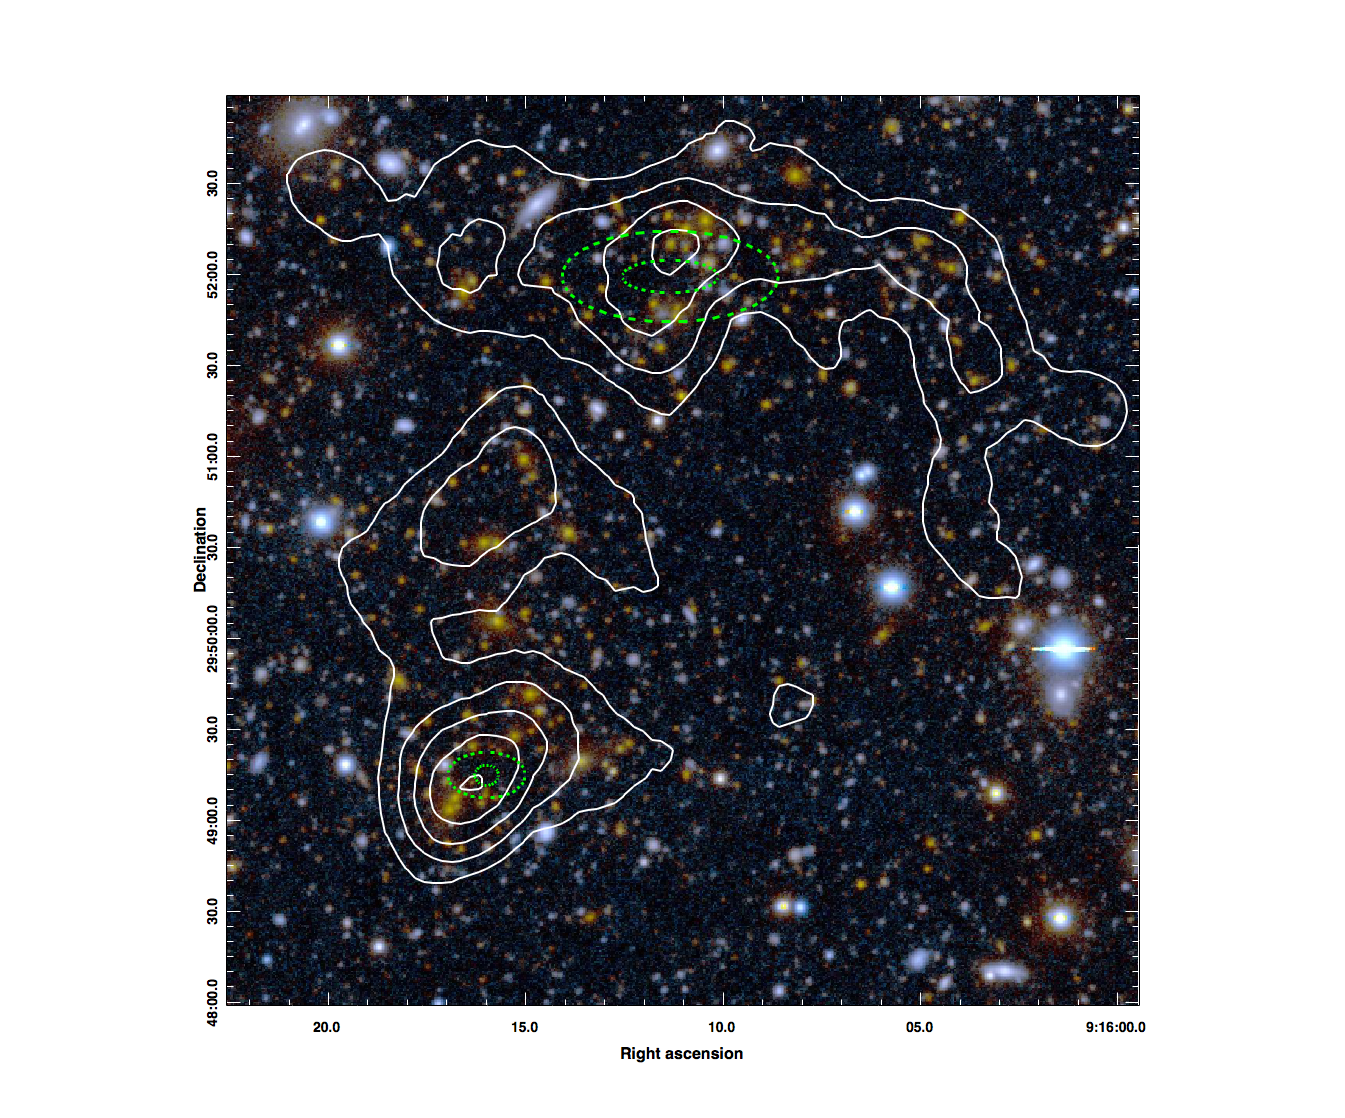
\includegraphics[width=5in]{Chapter4/DLScolor_wGalDenCon.png}
\caption[Musket Ball Cluster galaxy number density map including spectroscopic redshift information.]{
DLS composite $BVR$ color image of the Musket Ball Cluster showing  the galaxies of the two subclusters (predominately orange). 
This figure is similar to Figure \ref{fig2}, however the white contours representing the number density of galaxies now include both spectroscopic and photometric redshift information.
All (117) with galaxies spectroscopic redshift within three times the velocity dispersion of each subcluster were given a weight of 1.
All (270) galaxies without a spectroscopic redshift but with $z_{\rm phot}=0.53\pm0.1$ (the cluster redshift $\pm\sigma_{z_{\rm phot}}$) were given a weight of 0.63.
The photometric redshift sample weight is based on the empirically determined cluster membership purity of this sample, as determined from our magnitude limited spectroscopic survey of the cluster.
The contours begin at $\sim$200 galaxies\,Mpc$^{-2}$ with increments of $\sim$50 galaxies\,Mpc$^{-2}$.
The dashed green ellipses show the approximate galaxy centroid 68\% and 95\% confidence limits for each subcluster.
}
\label{figure:GalDenMap_withspec}
\end{figure}

Finally it is worth noting that  we have disregarded the centroid error associated with subcluster to subcluster galaxy membership contamination (see \S\ref{section:ClusterMembership}).
This is a potentially important source error and could cause a bias in the centroid estimates of each subcluster towards the direction of the other subcluster.
To the best of our knowledge no-one has performed studies investigating this particular bias. As such, accounting for and correcting such a bias in the Musket Ball Cluster (and other dissociative mergers) will require a significant amount of investigation and is beyond the scope of this current dissertation.
One could consider something like the multicomponent joint fitting method of \citet{Walker:2011eg}.


%--------------------------------------------------------
%--------------------------------------------------------
%--------------------------------------------------------
\section{Gas Location}\label{section:GasLocation}

When estimating the central gas centroid (black circles of Figure \ref{figure:XrayCentroid}), all detected point sources (small green circles with red dashes of Figure \ref{figure:XrayCentroid}) are excluded.
Additionally the diffuse southern gas concentration is excluded (large green rectangular box of Figure \ref{figure:XrayCentroid}).
The remaining X-ray photons in the green semicircle are then used to estimate the gas centroid of the central concentration, using  the \textit{dmstat} function of the Chandra Interactive Analysis of Observations (CIAO) software package.
We note that adaptive smoothing can introduce some artifacts to the image, however we find excellent agreement between the centroid of the smoothed image (black `x' in Figure \ref{figure:XrayCentroid}) and the centroid of the unsmoothed image (black circles of Figure \ref{figure:XrayCentroid}) suggesting that the smoothed map provides a reasonable representation of the gas.

We find that the central gas concentration centroid ($09\fh16\fm13\fs\pm8\fs, 29\fdg50\farcm55\farcs\pm9\farcs$) is offset $5.0\farcs$ from the peak of the gas distribution ($09\fh16\fm15\fs\pm5.5\fs, 29\fdg50\farcm59\farcs\pm5.0\farcs$).
Both are significantly offset between the northern and southern galaxy and WL concentrations.

\begin{figure}
\centering
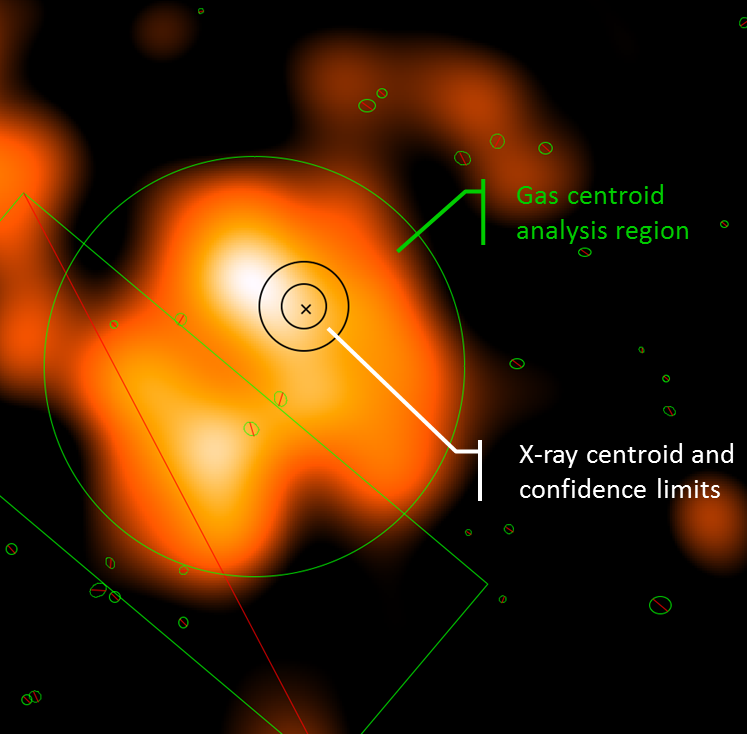
\includegraphics[width=5in]{Chapter4/XrayCentRegions_reformat.png}
\caption[Musket Ball Cluster X-ray map with estimated centroid.]{
Chandra ACIS-I 40\,ks adaptively smoothed X-ray image of DLSCL J0916.2+2951 (the same as Figure \ref{figure:MusketBallXray}).
The green circles and boxes are the SAOImageDS9 inclusion and exclusion regions used in conjunction with the Chandra Interactive Analysis of Observations (CIAO) software package.
The unsmoothed central gas centroid 68\% and 95\% confidence intervals are represented by the black circles.
The smoothed central gas centroid is represented by the black `x'.
The image field-of-view is the same as Figure \ref{fig1}.
}
\label{figure:XrayCentroid}
\end{figure}

%-------------------------------------------------------
%-------------------------------------------------------
%-------------------------------------------------------

\section{Weak Lensing Location}\label{section:WLLocation}

As discussed in Chapter \ref{chapter:1} the best means of determining the location of the DM is with gravitational lensing since it is capable of mapping the total projected mass, which is predominately DM.
Generically the major sources of error when mapping the location of DM with WL are galaxy shape measurement error, intrinsic ellipticity of galaxies, projected line-of-sight massive structures, and discrimination of foreground and cluster galaxies from the lensed source population of galaxies.
These sources of error are discussed at great length elsewhere \citep[see e.g.][]{Schneider:2006tp, Dietrich:2011gs} and for the specific case of the Musket Ball Cluster in Chapter \ref{chapter:2}.
However there are a number of sources of error unique to dissociative mergers.
First the DM mass of the one subcluster will cause a directional bias in the WL estimate of the DM location of the other subcluster away from the true DM location towards the first subcluster.
Similarly the dissociated gas will cause a directional bias of the WL estimated DM location of one subcluster towards the center of the merger.
Both of these directional biases will mimic the expected affect of SIDM.
In this section we will review how we account for the generic WL errors and go into detail on how we estimate the directional biases to the DM centroid location.

\subsection{Generic WL Errors}

Details of the galaxy shape measurement for the Musket Ball Cluster are discussed in Chapter \ref{chapter:2}.
We account for the effects of shape measurement and intrinsic ellipticity errors on the WL location in much the same way as we estimate the signal-to-noise of our WL mass maps as a whole (see \S\ref{section:Chap2WL}).
This is done by generating 10,000 bootstrap realizations of the HST WL mass map, where each realization is created with a random sample of the lensed source galaxy population.
Then just as we do for the galaxy centroid location (see \S\ref{section:GalaxyLocation}) we iteratively determine the centroid of each subcluster in each bootstrap realization of the mass map.
The distributions of centroids in these bootstrap realizations is then used to  calculate bias-corrected percent confidence limits \citep{Beers:1990kg} of the marginalized right ascension and declination distributions.

As for the effects of projected line of sight structures, \citet{Dietrich:2011gs} find that in their simulations line-of-sight structures contribute slightly ($\sim$2'') to the lensing centroid uncertainty.
Furthermore we find no evidence of significant line of sight structures using our full sample of 654 spectroscopic redshifts (with uniform selection over $0<z<1.0$) as well as photometric redshifts (see further discussion in Chapter \ref{chapter:2}). 
Based on our findings we confidently rule out any line of sight structures with $M_{\rm 200}\gtrsim1\times10^{12} M_\odot$.
Any undetected structure will have negligible impact on the offset.

Just as redshift uncertainties affect the galaxy centroid estimate (see \S\ref{section:ClusterMembership}) they too affect the WL centroid estimate.
However unlike with the galaxy centroid estimate, spectroscopic redshifts help very little to improve the WL centroid estimate.
This is because most of the lensing information comes from the large number of faint ($R\gtrsim23$) galaxies that predominately make up the lensed source population.
There is negligible spectroscopic information available for this population. 
So we rely almost entirely on photometric magnitude, color, and redshift information.
Fortunately WL is not quite as sensitive to these errors as the galaxy membership determination due to the relatively broad lensing redshift kernel (see Equation \ref{equation:WLshear})\footnote{However as previously noted the breadth of this WL kernel is also a hindrance when determining the WL centroid since line-of-sight massive structures can induce additional noise in WL centroid estimate of the DM halo centroid.}.
However it is still important to properly account for the inherently large errors associated with photometric redshifts.
The full $p(z)$ tomographic lensing method introduced in \S\ref{section:Chap2WL} is designed to do just that.
The method's effectiveness has recently been show in the case of Abell 781 (Wittman, Dawson, \& Benson, 2013) where it increased the signal-to-noise of the Abell 781-D subcluster by $\sim$40\%, thereby resolving the missing WL mass mystery \citep{Cook:2012ka}.


\subsection{Noise and Systematic effects}

duffy et al concentration scaling relation

\textbf{(1)} We model the surface mass density of the north and south subclusters with three NFW halos using masses determined by \citet{Dawson:2012dl}. We recursively estimate the centroid of this model and find an offset $3.4''$ from the true centroid towards the northern subcluster. 


\textbf{(2)} We then combine estimated surface mass densities of the
Central and South gas concentrations with the previous DM surface
densities from step (1) which results in a $7.6''$ centroid offset (dashed red curve of Figure \ref{fig3}).  
For perspective, if we double the gas mass the total offset increases to $10''$, or if we account for the uncertainty in our distribution of the gas mass the modeled centroid offset ranges from $3.4''$ to $9.4''$ (light red region of Figure \ref{fig3}). 
With the proposed Chandra observations we can better constrain the gas mass by approximately a factor of 10 and constrain the distribution of the gas mass so that the resulting uncertainty in the modeled centroid offset is reduced by at least a factor of 2 (dark red region of Figure \ref{fig3}).



\section{Gas--Weak Lensing Offset}\label{section:GasWLOffset}

%copied from \citep{Dawson:2012dl}
The peak of the gas distribution ($09\fh16\fm15\fs\pm5.5\fs, 29\fdg50\farcm59\farcs\pm5.0\farcs$) derived from X-rays is offset $1.4\arcmin\pm0.49$ from the North HST WL mass peak ($09\fh16\fm10\fs\pm30\fs, 29\fdg52\farcm10\farcs\pm30\farcs$), and $1.4\arcmin\pm0.14$ from the South HST WL mass peak ($09\fh16\fm15\fs\pm8.0\fs, 29\fdg49\farcm34\farcs\pm6.9\farcs$), and is located near a local minimum in the mass (see Figure \ref{fig3}).
Given the significant offset between the WL and gas locations we are able to use the first method of \citet{Markevitch:2004dl} and place a rough limit on the DM self-interaction cross-section, $\sigma_{\rm DM}$.
This method compares the scattering depth of the dark matter, $\tau_{\rm DM}=\sigma_{\rm DM}m^{-1}_{\rm DM} \Sigma_{\rm DM}$, with that of the ICM gas, $\tau_{\rm ICM}\approx 1$, where $m_{\rm DM}$ is the DM particle mass and $\Sigma_{\rm DM}$ is the surface mass density of the DM particles.
$\Sigma_{\rm DM}$ is approximately the WL measured surface mass density, $\Sigma$, since $\sim80\%$ of a typical cluster's mass is DM \citep{Diaferio:2008js}.
For ease of comparison with the results of \citet{Markevitch:2004dl} and \citet{Merten:2011gu} we examine the surface density averaged over the face of the subcluster within $r$=125\,kpc, which is $\Sigma\approx0.15$\,g\,cm$^{-2}$; thus we find $\sigma_{\rm DM} m_{\rm DM}^{-1} \lesssim 7$\,cm$^2$\,g$^{-1}$. 


\begin{figure}
\centering
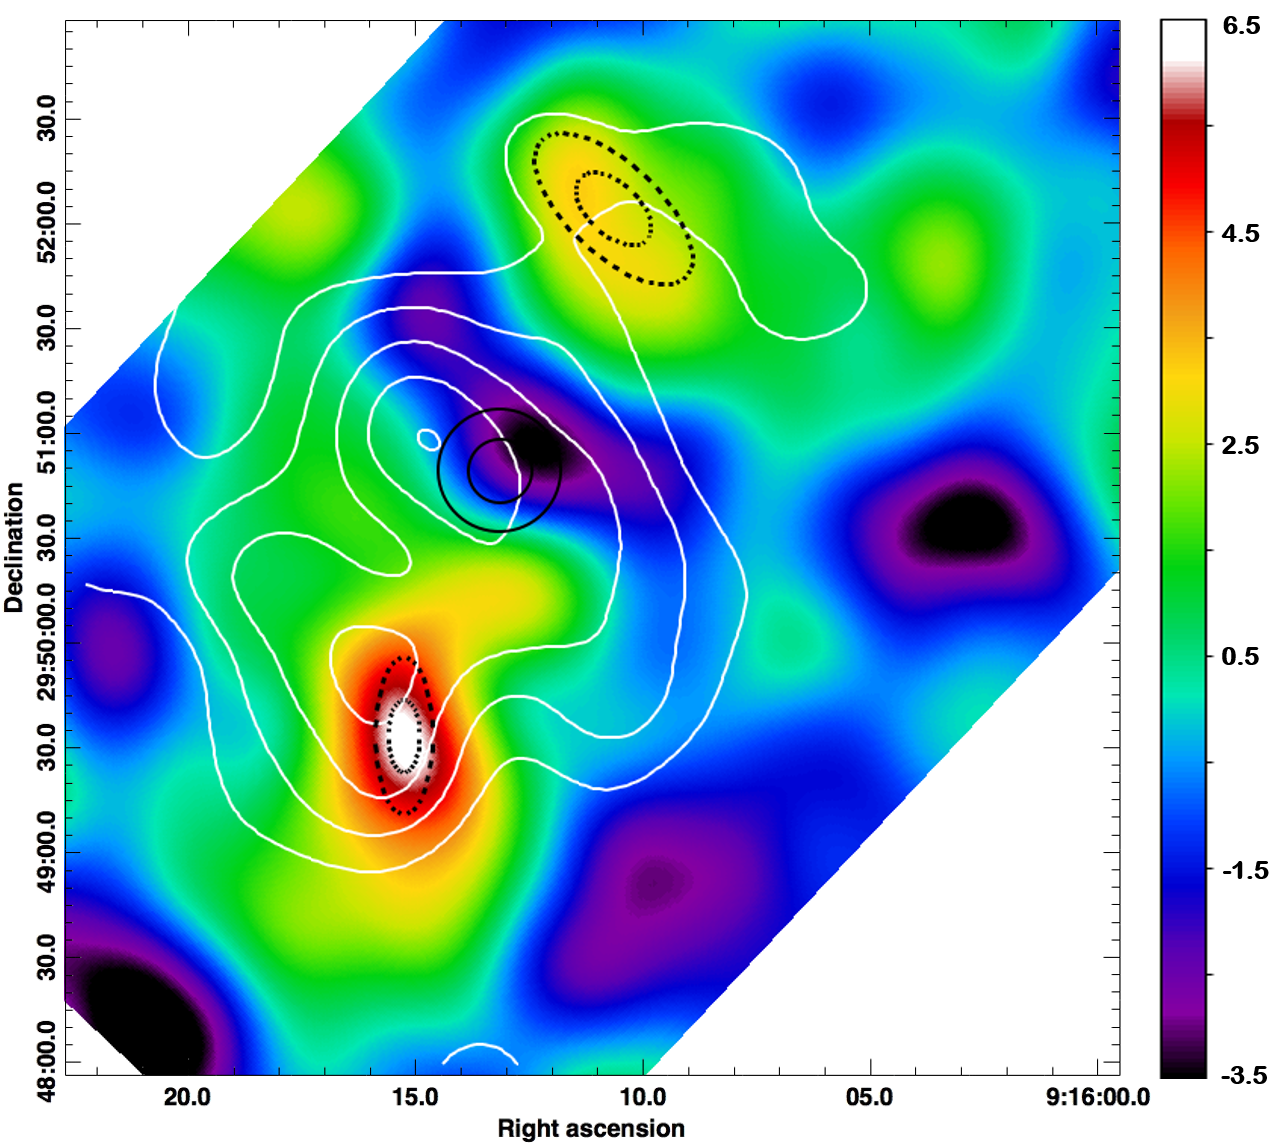
\includegraphics[width=5in]{Chapter4/LensingXrayOverlay.png}
\caption[Musket Ball Cluster weak lensing signal-to-noise map with X-ray map overlay, including centroid locations.]{
HST space-based WL mass signal-to-noise map of the Musket Ball Cluster with the X-ray distribution overlay (white contours).
The 68\% and 95\% centroid confidence intervals are shown for the north and south subcluster WL centroids (dashed black ellipses) as well as the central gas distribution (solid black ellipses).
The majority of the cluster gas is centered $\sim1.4\arcmin$ between the North and South subclusters.
}
\label{figure:LensingXrayOverlay}
\end{figure}


\section{Galaxy--Weak Lensing Offset}\label{section:GalaxyWLOffset}

The offset is now 20.5''

Section text

\begin{figure}
\centering
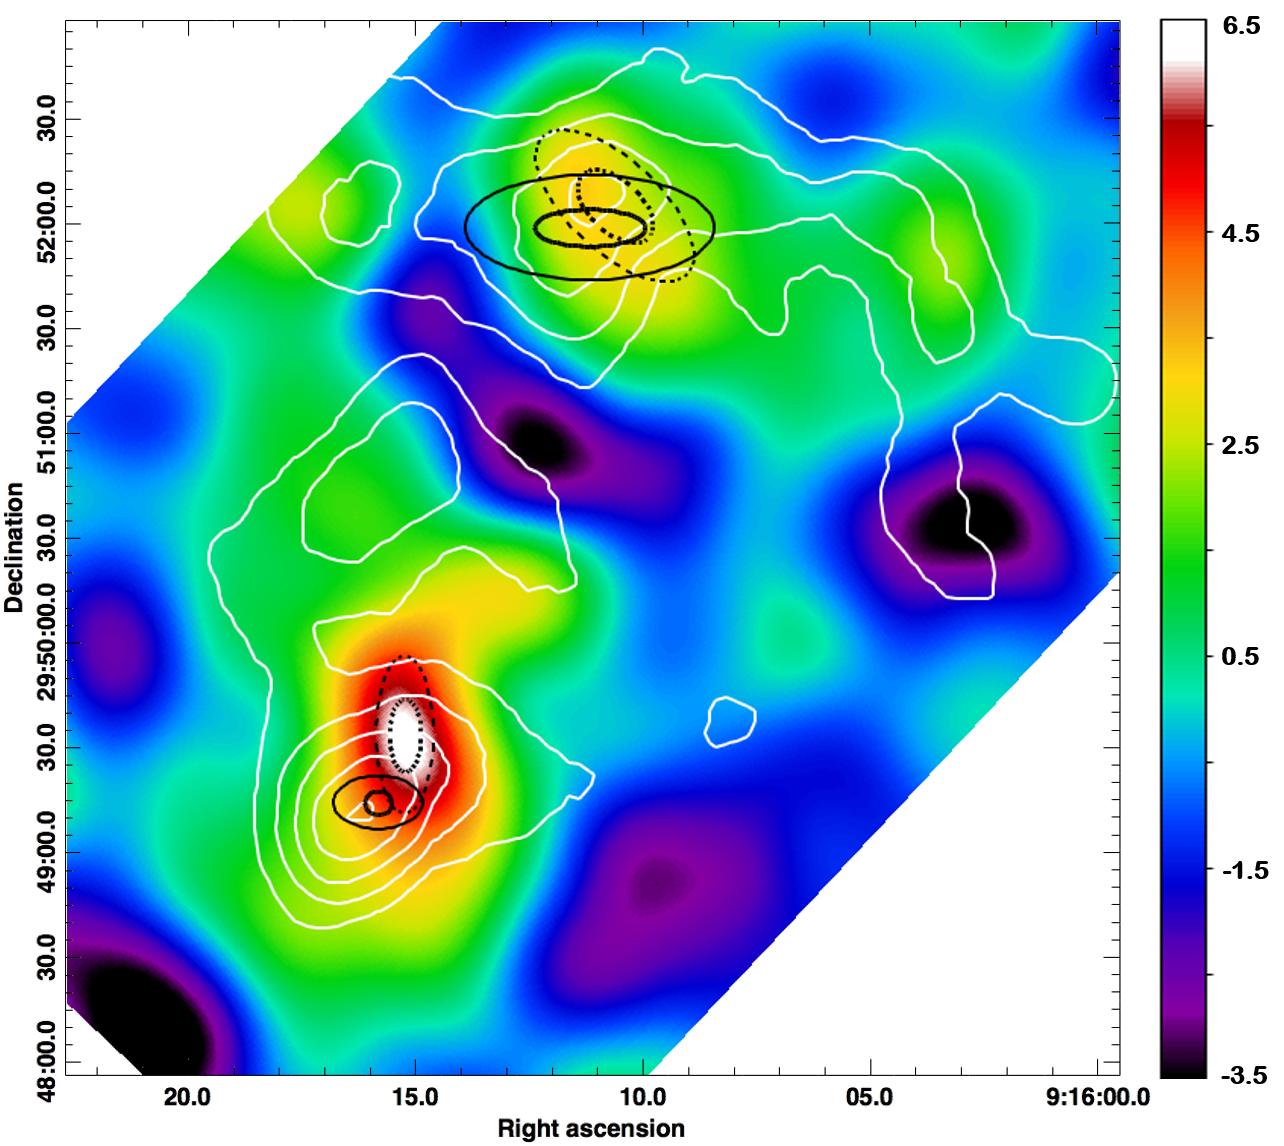
\includegraphics[width=5in]{Chapter4/LensingGalaxyOverlay.png}
\caption[Musket Ball Cluster weak lensing signal-to-noise map with galaxy number density map overlay, including centroid locations.]{
HST space-based WL mass signal-to-noise map of the Musket Ball Cluster with the spectroscopic and photometric redshift based galaxy number density overlay (white contours).
The 68\% and 95\% centroid confidence intervals are shown for the north and south subcluster WL centroids (dashed black ellipses) as well as north and south galaxy number density centroids (solid black ellipses).
Note the 20.5'' offset between the galaxies and the WL mass in the South subcluster.
}
\label{figure:LensingGalaxyOverlay}
\end{figure}



\begin{figure}
\centering
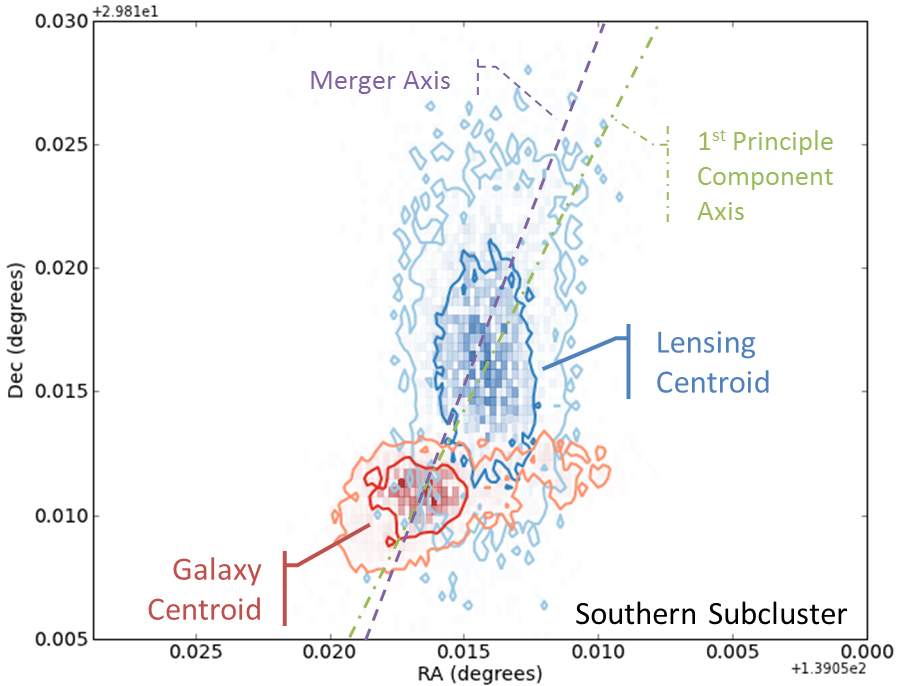
\includegraphics[width=5in]{Chapter4/AnalysisFiles/southcentroids_histplot2d_reformat.png}
\caption[Musket Ball southern subcluster galaxy and weak lensing centroid spatial distribution.]{
Musket Ball southern subcluster WL (blue) and galaxy number density (red) centroid probability density distribution functions constructed from 10,000 respective bootstrap realizations.
The 68\% (dark contours) and 95\% (light contours) confidence intervals are shown for each.
The region shown is 1.5' by 1.5' ($567\times 567\,kpc^2$ at $z$=0.53).
The first principle component axis of two distributions (dot-dashed green line) has a position angle of 159 degrees, this close to the 153 degree position angle of the merger axis of the cluster (dashed purple line; as inferred from a line intersecting the two galaxy centroids) .
}
\label{figure:CentroidDist_South}
\end{figure}

Both centroids in the northern subcluster are less well defined than the centroids in the southern subcluster.
This is likely due to the northern subcluster being approximately half as massive as the northern subcluster.


\begin{figure}
\centering
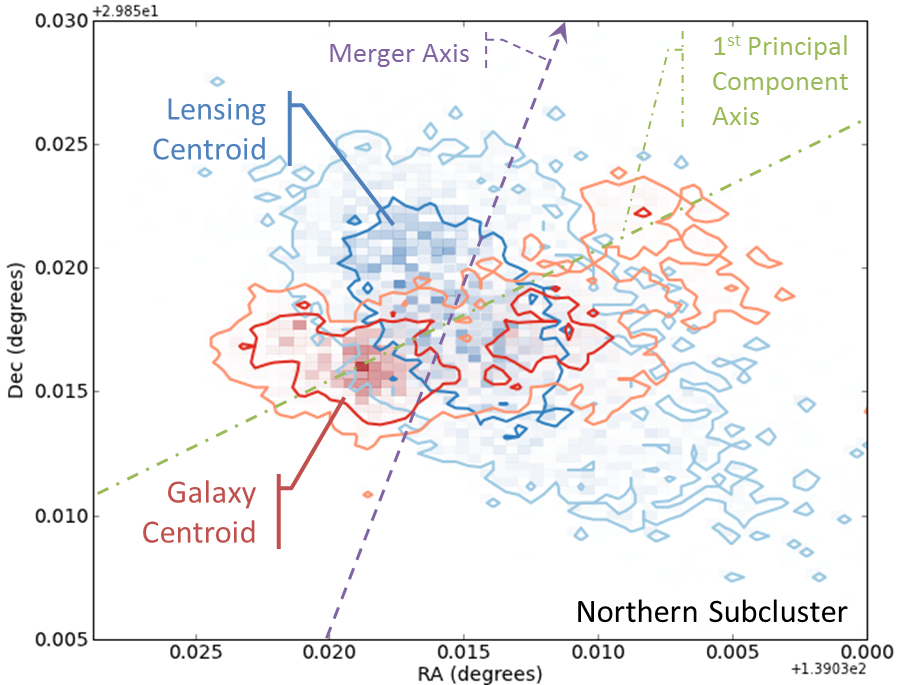
\includegraphics[width=5in]{Chapter4/AnalysisFiles/northcentroids_histplot2d_reformat.png}
\caption[Musket Ball northern subcluster galaxy and weak lensing centroid spatial distribution.]{
Musket Ball northern subcluster WL (blue) and galaxy number density (red) centroid probability density distribution functions constructed from 10,000 respective bootstrap realizations.
The 68\% (dark contours) and 95\% (light contours) confidence intervals are shown for each.
The region shown is 1.5' by 1.5' ($567\times 567\,kpc^2$ at $z$=0.53), the same scale as Figure \ref{figure:CentroidDist_South}.
The merger axis of the cluster (as inferred from a line intersecting the two galaxy centroids) is plotted as a dashed purple line.
Unlike the southern subcluster (Figure \ref{figure:CentroidDist_South}) there does not appear to be a significant offset between between the locations.
Both centroids in the northern subcluster are less well defined than the centroids in the southern subcluster; most notably the galaxy density centroid which appears bimodal.
}
\label{figure:CentroidDist_North}
\end{figure}

Perhaps include some figures discussing systematic offset tests.

The statistical question we pose is:
If the WL and galaxy parent distributions coincide how often would one expect the observed offset of the galaxies leading the WL along the mergers axis\footnote{This is a one-tailed test}.
Assuming the two centroids are expected to coincide in the CDM scenario then the complement of the previous probability is the confidence that $\sigma_{\rm DM}>0$.
Also assuming no systematic errors or random noise not captured by the bootstrap analysis.

\begin{figure}
\centering
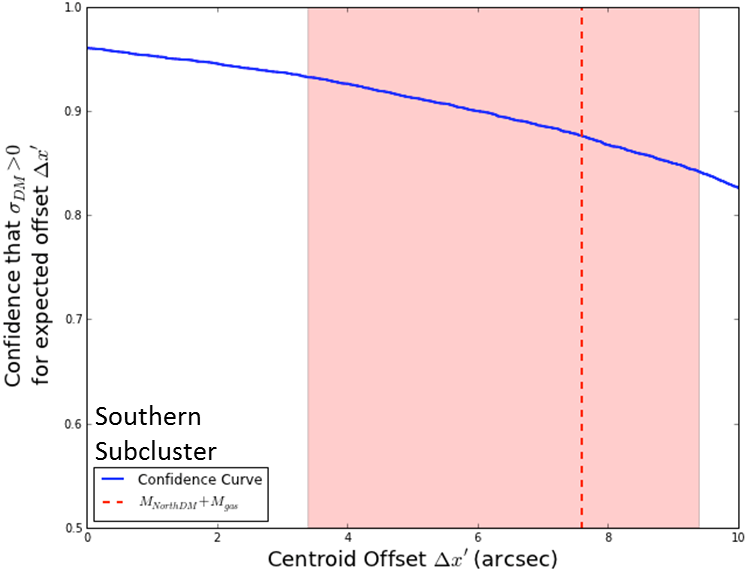
\includegraphics[width=5in]{Chapter4/AnalysisFiles/GalDenVsHSTWL_pzpen_delxPC_south_reformat.png}
\caption[Musket Ball southern subcluster galaxy and weak lensing centroid offset significance.]{

The galaxy-WL centroid offset is measured along the merger axis direction ($x'$) with positive offsets being when the galaxies lead the DM (as expected in the case of SIDM).
}
\label{figure:CentroidSignificance_South}
\end{figure}

\begin{figure}
\centering
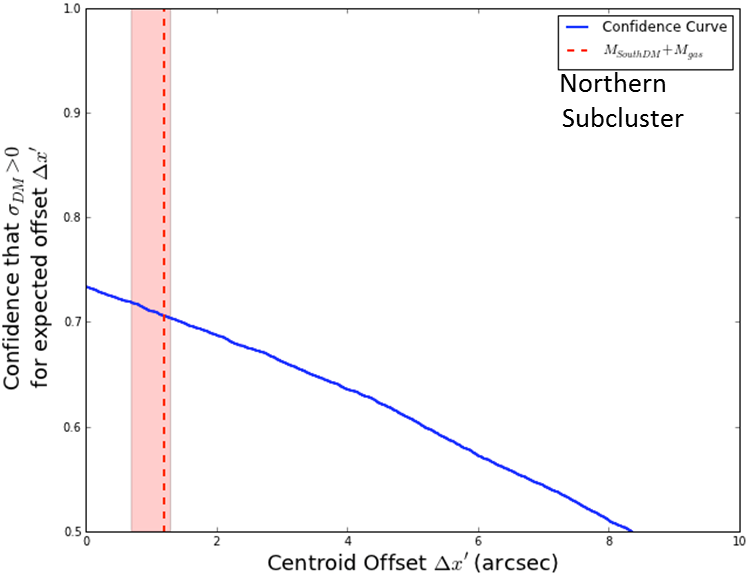
\includegraphics[width=5in]{Chapter4/AnalysisFiles/GalDenVsHSTWL_pzpen_delxPC_north_mergeraxis_reformat.png}
\caption[Musket Ball northern subcluster galaxy and weak lensing centroid offset significance.]{
}
\label{figure:CentroidSignificance_North}
\end{figure}

\section{Discussion}

Discussion text

simulations to study the directional bias of galaxy centroid and WL centroid measurements in dissociative mergers


note importance of fitting both subcluster simultaneously

better modeling of the gas mass and its effect on the systematic centroid offset

note alternatives to centroid estimation, both in measuring the galaxy-dark matter offset as well as just other ways to measure the galaxy centroid, e.g. \citep{Randall:2008hs}

note other means of estimating the offset independent of centroid measurements

For galaxy centroid consider other measurements of the galaxy population location, other than number density, for example weighting the galaxies by luminosity or stellar mass.

Discuss work of \citep{Kahlhoefer:2013wp}

One thing that hasn't been discussed is the typical intrinsic scatter in the lensing centroid. Reference the George, M. work noting that they find that the galaxy center is often $\sim$50kpc from the lensing center. There are a number of problems with directly translating this result to the work discussed here. Since they were dealing with groups of galaxies (typically $\sim$1 order of magnitude less massive and $\sim$1 order of magnitude fewer galaxies than galaxy cluster) they 1) have fewer galaxies with which to beat down the Poisson noise of the centroid estimate, 2) their result is based on which center maximizes the lensing signal of 129 galaxy groups. 

importance of using multiple systems (beat down intrinsic scatter in galaxy-DM offset as well as other sources of noise)

importance of simulations, not only for quantifying the cross-section constraints but also for studying systematic effects (e.g. the intrinsic galaxy-DM offset, both in relaxed cluster as well as merging clusters)

tweak the cluster membership criteria in order to simultainously minimize the joint uncertainty due to cluster membership noise and Poisson noise of the centroid estimate.

\section{Conclusions}

Conclusion text

\textbf{acknowledgements:}
Acknowledgment text
%\end{acknowledgements}

%\bibliographystyle{apj}
%\bibliography{Chapter1/chapter1}{}



%% The References
%\bibliographystyle{thesis}
%\begin{singlespacing}
%  \bibliography{Chapter3/chapter3}
%\end{singlespacing}
